\section{Zielsetzung}
\label{sec:zielsetzung}

In diesem Versuch werden mittels $\gamma$-Spektrometrie die Energiespektren verschiedener
$\gamma$-Strahler durch einen Reinst-Germanium-Detektor ausgemessen.
Es werden insgesamt vier verschiedene Proben untersucht.
Zu Beginn wird die Theorie hinter der Funktionsweise eines Germanium-Detektors
beschrieben. Danach wird das Vorgehen der Messung erläutert, sowie der Aufbau
skizziert. Anschließend werden die gemessenen Spektren aufgeführt, ausgewertet und
abschließend diskutiert.

\section{Theorie}
\label{sec:theorie}

Im Folgenden wird die Funktionsweise eines Germanium-Detektors beschrieben,
wobei zunächst allgemein die Wechselwirkung von $\gamma$-Quanten mit Materie
betrachtet wird.

$\gamma$-Quanten wechselwirken mit Materie grundlegend über drei verschiedene Effekte.
Es handelt sich dabei um den Photoeffekt, die Compton-Streuung und die Paarbildung.
Die verschiedenen Effekte haben unterschiedliche Wirkungsquerschnitte $\sigma$,
welche darüber hinaus noch von der Enenergie $E_{\gamma}$ der $\gamma$-Quanten abhängig sind.
Anschaulich kann der Wechselwirkungsquerschnitt als eigenommene Fläche
eines Elektrons aufgfasst werden, welche nicht von den $\gamma$-Quanten durchdrungen
werden kann, also auf der $\gamma$-Quanten absorbiert werden.
Die Extinktion einer mit $N_0$  $\gamma$-Quanten eintreffenden Population mit der
Eindringtiefe $\symup{d}x$ wird aus
\begin{equation}
  \label{eqn:dgl_eindringtiefe}
  \symup{d}N = N_0n\sigma\symup{d}x
\end{equation}
hergeleitet. Dabei ist $n$ die Anzahl der Elektronen pro Volumen $V$.
Für einen Absorber mit
Dicke $D$ ergibt sich eine Verarmung der ursprünglichen Population $N_0$ auf $N(D)$
mit dem funktionalen Zusammenhang
\begin{equation}
  \label{eqn:eindringtiefe}
  N(D) = N_0\exp{(-n\sigma D)}.
\end{equation}
Der Exponent von~\eqref{eqn:eindringtiefe} wird als Extionsktionskoeffizienten
\begin{equation}
  \label{eqn:ext}
  \mu = n\sigma
\end{equation}
definiert.
Der reziproke Extinktionskoeffizient ist die mittlere Reichweite $\bar{x}$
von $\gamma$-Quanten in Materie.
\begin{equation}
  \bar{x} = \frac{1}{\mu}
\end{equation}
Eine Darstellung der auftretenden Extinktionskoeffizienten $\sigma(E_{\gamma})$ ist in
Abbildung~\ref{fig:crosssection} zu finden.

\begin{figure}
  \centering
  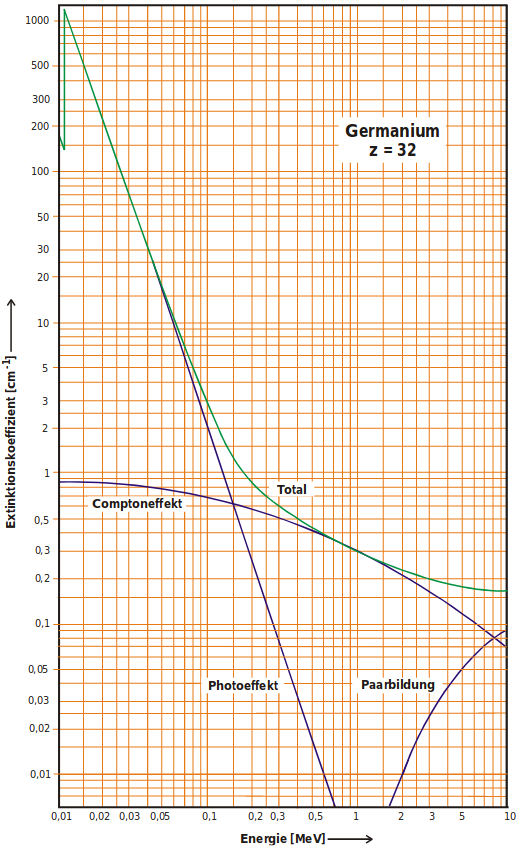
\includegraphics[width=0.9\textwidth]{Pics/crosssection.png}
  \caption{Extinktionskoeffizienten der verschiedenen Wechselwirkungen von $\gamma$-Quanten mit Germanium\cite{anleitung}.}
  \label{fig:crosssection}
\end{figure}

\subsection{Photoeffekt}
\label{subsec:photo}

Der Photoeffekt beschreibt die Wechselwirkung eines $\gamma$-Quants mit einem
Hüllenelektron der bestrahlten Materie.
Phänomenologisch kann der Photoeffekt über die folgende Gleichung erklärt werden.
\begin{equation}
  \label{eqn:photo}
  \gamma + \ce{Atom -> Atom^+} + e^-.
\end{equation}
Somit beschreibt der Photoeffekt die Ionisation eines Atoms.
Das eingehende $\gamma$-Quant besitzt die Energie $E_{\gamma} > E\ua{B}$.
Dabei ist $E\ua{B}$ die Bindungsenergie des Elektrons an dem Atom.
Die Energiedifferenz zwischen $E_{\gamma}$ und $E\ua{B}$ trägt das Elektron in Form
von kinetischer Energie weg.
Das ausgelöste Elektron hinterlässt in dem Atom ein Loch, welches durch ein Elektron
aus einer höheren Schale gefüllt wird. Die dabei frei werdende Energie
liegt typischerweise im Bereich der Röntgenstrahlung. In guter Näherung kann angenommen
werden, dass diese Röntgen-Quanten den Absorber nicht verlassen.
Das bedeutet bei dem Photoeffekt ist davon auszugehen, dass die vollständige
Energie des $\gamma$-Quants im Absorber verbleibt.
Aufgrund dieser Tatsache, kann direkt auf
den Strahler zurückgeschlossen werden, da die Energie der emitierten $\gamma$-Quanten
eine charakteristische Größe des Strahles ist.

Der Wirkungsquerschnitt des Photoeffektes ist für den im Versuch auftretenden
Energiebereich approximativ mit
\begin{equation}
  \label{eqn:crosssection_photo}
  \sigma\ua{Ph} \sim \frac{z^\alpha}{E^{\num{3,5}}}
\end{equation}
gegeben. $z$ entspricht der Kernladungszahl der wechselwirkenden Materie und $\alpha$
ist eine Exponent mit $4 < \alpha < 5$\cite{anleitung}.

\subsection{Compton-Streuung}
\label{subsec:compton}

Der Compton-Effekt beschreibt die Streuung von $\gamma$-Quanten an freien Elektronen
und wird durch folgende Gleichung beschrieben.
\begin{equation}
  \label{eqn:compton}
  \gamma + e^- \ce{->} \gamma '+ (e^-)'
\end{equation}
Gleichung~\eqref{eqn:compton} sagt aus, dass ein Energieübertrag zwischen dem
$\gamma$-Quant und dem Elektron $e^-$ stattfindet.
Der Prozess ist in Abbildung~\ref{fig:compton} schematisch illustriert.

\begin{figure}
  \centering
  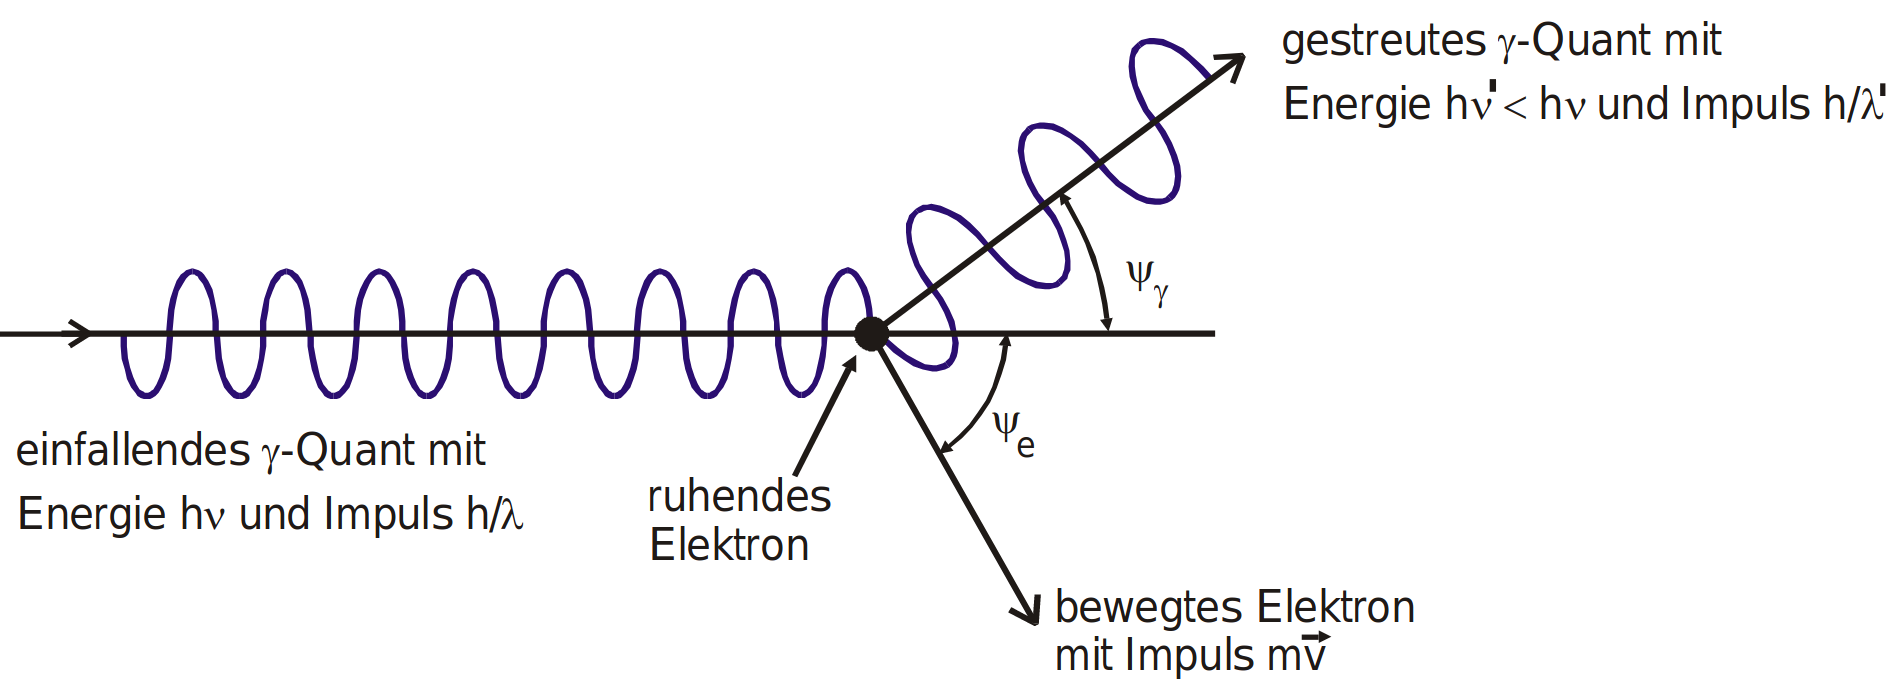
\includegraphics[width=0.9\textwidth]{Pics/compton.png}
  \caption{Schematische Darstellung der Compton-Streuung. $\Psi_\gamma$ ist der Streuwinkel des
  $\gamma$-Quants und $\Psi_{e^-}$ ist der Streuwinkel des gestoßenen Elektrons\cite{anleitung}.}
  \label{fig:compton}
\end{figure}

Die Impuls- und Energieerhaltung eines inelastischen Stoßes führen auf eine
$\gamma$-Quantenergie nach der Streuung $E_{\gamma}'$ von
\begin{equation}
  \label{eqn:comton_E_gamma}
  E_\gamma ' = E_\gamma\frac{m_0c^2}{m_0c^2 + E_\gamma\left(1 - \cos{(\Psi_\gamma)}\right)}.
\end{equation}
Die Energie des Elektrons nach der Streuung $E_{e^-}'$ ist gegeben durch
\begin{equation}
  \label{eqn:comton_E_el}
  E_{e^-}' = E-\gamma - E_\gamma ' = \frac{E_\gamma^2\left(1 - \cos{(\Psi_\gamma)}\right)}{m_0c^2 + E_\gamma\left(1 - \cos{(\Psi_\gamma)}\right)}.
\end{equation}
Der maximale Energieübertrag ist somit gegeben für $\Psi_\gamma = \SI{180}{\degree}$,
was einer Rückstreuung entspricht. Der Bereich bei diesem Streuwinkel wird
im Energiespektrum als Compton-Kante bezeichnet (vgl. Kapitel~\ref{subsec:energiespektrum}).
Der Wechselwirkungsquerschnitt der Compton-Streuung $\sigma_{Co}$
wird in Quelle~\cite{anleitung} angegeben mit
\begin{equation}
  \label{eqn:crosssection_compton}
  \sigma\ua{Co} = \frac{3}{4}\sigma\ua{Th}\left(\frac{1+\epsilon}{\epsilon^2}\left[\frac{2 + 2\epsilon}{1+2\epsilon} - \frac{1}{\epsilon}\ln{(1+2\epsilon)}\right] + \frac{1}{2\epsilon}\ln{(1+2\epsilon)}-\frac{1+3\epsilon}{(1+2\epsilon)^2}\right).
\end{equation}
Dabei ist $\sigma\ua{Th} = \frac{8}{3}\pi\left(\frac{e_0}{4\pi\epsilon_0 c^2m_0}\right)$
der Thomsonsche Streuquerschnitt und $\epsilon = \frac{E_{\gamma}}{m_0c^2}$.

\subsection{Paarbildung}
\label{subsec:paar}

Die Paarbildung tritt erst ab einer $\gamma$-Quantenergie von $E\gamma > 2m_0c^2$
auf. Der Prozess kann durch eine Gleichung der Form
\begin{equation}
  \label{eqn:paar}
  \gamma + \ce{Atom -> Atom} + e^+ + e^-
\end{equation}
erklärt werden. Aus Impulserhaltungsgründen ist die Energie des $\gamma$-Quants
auf beide Leptonen gleichmäßig aufgeteilt.
Anstelle des Atoms in Gleichung~\ref{eqn:paar} kann auch ein Elektron als Stoßpartner
fungieren, wobei die Paarbildung an Elektronen aufgrund einer höheren Schwellenenergie,
welche aus der geringeren Masse resultiert, unwahrscheinlicher ist.
Es wird nicht in jedem Fall die gesamte Energie eines einfallenden $\gamma$-Quants
im Absorber deponiert. Das erzeugte Positron rekombiniert mit einem Elektron
des Absorbers, wobei aus Impulserhaltungsgründen zwei Photonen entstehen.
Mit einer endlichen Wahrscheinlichkeit kann eines der beiden, oder beide
Photonen nicht wieder mit dem Absorber wechselwirken und
den Detektor ohne Energiedeponierung verlassen. Verlässt nur eines Photonen
den Detektor entsteht in dem Energiespektrum der sogenannte Single-Escape-Peak
und verlassen beide Photonen den Absorber entsteht der sogenannte
Double-Escape-Peak.
Der Wechselwirkungsquerschnitt der Paarbildung wird in der Referenz~\cite{anleitung}
für zwei verschiedene Fälle angegeben. Zum einen für vollständige
Abschirmung des Coulomb-Feldes, also wenn die Paarbildung
außerhalb der Elektronenhülle stattfindet und zum anderen für
eine verschwindende Abschirmung, wenn die Paarbildung in Kernnähe stattfindet.

Für den Fall vollständiger Abschirmung ergibt sich
\begin{equation}
  \label{eqn:crosssection_paar_abschirmung}
  \sigma\ua{Pa} = \alpha r\ua{e}^2z^2\left(\frac{28}{9}\ln{\left(\frac{183}{\sqrt[3]{z}}\right)} - \frac{2}{27}\right),
\end{equation}
und für den Fall verschwindender Abschirmung ergibt sich
\begin{equation}
  \label{eqn:crosssection_paar_no_abschirmung}
  \sigma\ua{Pa} = \alpha r\ua{e}^2z^2\left(\frac{28}{9}\ln{(2\epsilon)} - \frac{218}{27}\right),
\end{equation}
mit dem klassischen Elektronenradius $r_e = \frac{e_0}{4\pi\epsilon_0c^2m_0}$.

\FloatBarrier

\subsection{Wirkungsweise eines Reinst-Germanium-Detektors}
\label{subsec:wirkungsweise}
Germanium ist ein indirekter Halbleiter, weshalb ein Reinst-Germanium-Detektor
zu den Halbleiter-Detektoren gezählt wird.
Indirekte Halbleiter zeichnen sich dadurch aus, dass der geringste Abstand zwischen
Valenz- und Leitungsband
nicht direkt über dem $\su{\Gamma}$-Punkt liegt, sondern verschoben ist.
Aus diesem Grund wird für den Übergang eines Elektrons von dem Valenz-
in das Leitungsband ein zusätzliches Phonon benötigt, weshalb die
Anregungsenergie um ein Vielfaches größer ist als die eigentliche Bandlücke.

Halbleiter-Detektoren sind prinzipiell wie $pn$-Dioden aufgebaut (vgl. Abbildung~\ref{fig:pndiode}).
$p$ und $n$ weisen auf die Dotierung des Halbleiters hin.
Bei $p$-dotierte Halbleiter werden Elektronen-Akzeptoren in den Halbleiter
eingebracht und bei $n$-dotierten Halbleitern werden Elektronen-Donatoren
eingebracht.
Im Bereich der Kontaktstelle zwischen $p$- und $n$-dotierten Halbleitern
entsteht eine Grenzschicht, in der die Donator-Elektronen mit den Akzeptor-Elektronen
rekombinieren. Diese Grenzschicht wird als Verarmungszone bezeichnet.
Die $p$-Schicht und die $n$-Schicht bilden aufgrund ihrer unterschiedlichen
Dotierungen ein elektrostatisches Feld aus.
Auf die Verarmungszone einfallende $\gamma$-Quanten lösen durch die beschriebenen
Wechselwirkungsprozesse proportional zu ihrer deponierten Energie Elektronen aus.
Ein ausgelöstes Elektron hinterlässt eine positive Ladungslücke,
welche als Loch bezeichnet wird. Elektronen und Löcher diffundieren in dem
elektrostatischen Feld der $pn$-Diode zu den jeweiligen Elektroden und können dort
als Strom nachgewiesen werden.

Außerhalb der Verarmungszone werden in einem Halbleiterdetektor die Elektronen
und Löcher nicht schnell genug getrennt, sodass diese rekombinieren und nicht
an den Elektroden nachgewiesen werden können.
Aus diesem Grund ist es wichtig, die Verarmungszone möglichst auszuweiten,
damit möglichst viele $\gamma$-Quanten ihre vollständige Energie deponieren.
Die Größe der Verarmungsschicht hat aufgrund von~\eqref{eqn:eindringtiefe}
somit einen direkten Einfluss auf die Anzahl der $\gamma$-Quanten, die
ihre Gesamtenergie deponieren.
Das Ausweiten kann durch Anlegen einer äußeren Spannung, der sogenannten Sperrspannung
$U$ bewirkt werden.
Bei Temperaturen ungleich Null entstehen Leckströme, weshalb die Spannung
nicht beliebig groß sein kann. Leckströme entstehen beispielsweise durch Störstellen
oder durch das thermische Auslösen von Elektronen in dem Detektormaterial.
Durch aktives Kühlen des Detektors können Leckströme reduziert werden.

Darüber hinaus kann die Verarmungszone durch eine extrem asymmetrische Dotierung
vergrößert werden, also zum Beispiel $n\ua{D}\gg n\ua{A}$.
In diesem Fall erstreckt sich die Verarmungszone nahezu über die gesamte $p$-Schicht.
Es ist zu beachten, dass ein Detektor sogenannte Totbereiche beinhaltet, in denen
kein Teilchennachweis stattfindet. Durch mangelnde Kühlung kann der Totbereich,
der aufgrund der Lithium-Schicht entsteht, bei dem verwendeten Detektors vergrößert werden.
Die von außen aufgedampften Lithium-Atome (vgl. Kapitel~\ref{sec:aufbau}) können bei höheren Temeraturen
schneller in das Detektormaterial diffundieren, wodurch der Totbereich
ausgedehnt wird.

Mit Hilfe der beschriebenen Mittel kann die Verarmungszone in dem verwendeten
Reinst-Germanium-Detektor wenigen $\si{\micro\meter}$ auf
$d\approx\SI{3}{\centi\meter}$ ausgeweitet werden.
\begin{figure}
  \centering
  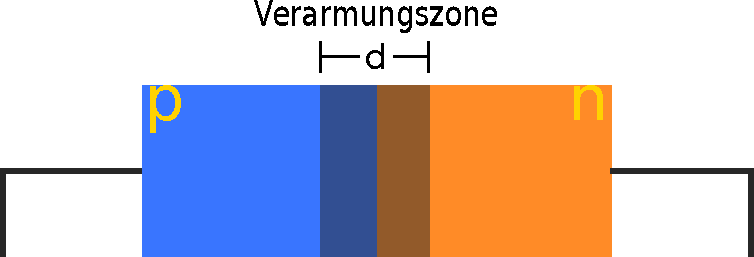
\includegraphics[width=0.8\textwidth]{Pics/pndiode.pdf}
  \caption{Schematische Abbildung einer $pn$-Diode mit einer Verarmungszone der Größe $d$.
  Das Anlegen einer Sperrspannung $U$ wird durch die eingezeichneten Elektroden angedeutet.}
  \label{fig:pndiode}
\end{figure}
\FloatBarrier
\subsection{Energieauflösung eines Halbleiter-Detektors}
\label{subsec:energieauflösung}

Die Energieauflösung ist eine charakteristische Eigenschaft eines Detektors.
Sie kann anhand der Halbwertsbreite $\Delta E_{1 / 2}$ einer Impulshöhenverteilung
definiert werden. Qualitativ sagt dieses Kriterium aus, wie nah zwei
Mittelwerte von gleichen Gaußverteilungen zusammenliegen dürfen um noch
eindeutig voneinander unterscheidbar zu sein. Dieses Kriterium ist in
Abbildung~\ref{fig:energieauflösung} veranschaulicht.
Die Energieauflösung von indirekten Halbleiter-Detektoren wird aufgrund der statistischen
Verteilung der $\gamma$-Quantenergie auf die Phononen- und Elektronen-Loch-Paar-Erzeugung
beeinträchtigt.
Wird eine Poisson-Verteilung der Elektronen-Loch-Paar-Erzeugung angenommen
ergibt sich eine Standardabweichung von
\begin{equation}
  \label{eqn:poisson}
  \sigma_{Poisson} = \sqrt{\bar{n}},
\end{equation}
mit $\bar{n}  = \frac{E_\gamma}{E\ua{E-L}}$ ($E\ua{E-L}$: Erzeugungsenergie eines Elektron-Loch-Paars).
Jedoch ist zu beachten, dass die Fluktuationen der Elektron-Loch-Paar-Erzeugung durch
Fluktuationen in der Phononenerzeugung teilweise kompensiert wird.
Diese Tatsache wird durch den Fano-Faktor $F < 1$ berücksichtigt.
\begin{equation}
  \label{eqn:fano}
  \Rightarrow \sigma = \sqrt{F\cdot\bar{n}}
\end{equation}
Für Germanium wird ein Wert von $F\ua{Ge}\approx \num{0.1}$ angegeben\cite{anleitung}.\\
Ist die Anzahl der Elektronen-Loch-Paar-Erzeugungen sehr groß,
geht die Poisson-Verteilung in eine Gaußverteilung über, für die sich bei $E_\gamma = \SI{500}{\keV}$
eine Halbwertsbreite von
\begin{equation}
  \label{eqn:halbwertsbreite}
  \Delta E_{1/2}(\SI{500}{\keV}) = \sqrt{8\ln{(2)}}\sqrt{F\cdot E_\gamma E\ua{E-L}} \approx \num{2,35} \sqrt{\num{0,1}E_\gamma E\ua{E-L}} \approx \SI{895}{\eV}
\end{equation}
ergibt.
In Tabelle~\ref{tab:E_aufloesung} ist die Energieauflösung nach Formel~\eqref{eqn:halbwertsbreite}
für verschiedene Materialien angegeben.
\begin{table}c
  \centering
  \caption{Energieauflösung für verschiedene Halbleitermaterialien nach Formel~\eqref{eqn:halbwertsbreite}
  mit den Werten aus~\cite{teilchendetektoren}.}
  \label{tab:E_aufloesung}
  \begin{tabular}{c S S S}
    \toprule
    {Material} & {Fano-Faktor} & {$E\ua{E-L} / \si{eV}$} & {$\Delta E_{1/2} / \si{keV}$} \\
    \midrule
    Si & 0,115 & 3,65 & 1,766 \\
    GaAs & 0,1 & 4,35 & 1,096 \\
    CdTe & 0,1 & 4,45 & 1,106 \\
    Diamond & 0,08 & 13,1 & 1,701 \\
    \bottomrule
  \end{tabular}
\end{table}

Durch Leckströme~$H\ua{I}$, Feldinhomogenitäten~$H\ua{E}$ und thermisches Rauschen
in dem Detektor und der Ausleseelektronik~$H\ua{R}$
wird die Energieauflösung weiter beeinträchtigt.
Damit ergibt sich die Gesamthalbwertsbreite eines realen Detektors zu
\begin{equation}
  \label{eqn:reale_energieauflösung}
  H^2\ua{ges} = \Delta E_{1/2}^2 + H^2\ua{I} + H^2\ua{E} + H^2\ua{R} .
\end{equation}
Elektronisches Rausch und das Ausbilden von Leckströmen können durch Kühlen
des Detektors verringert werden. Die Feldinhomogenitäten des
elektrostatischen Feldes des Detektors kann durch Erhöhen der
Sperrspannung verringert werden, wobei sich die Leckströme antiproportional dazu
verhalten. Daher gibt es einen optimalen Bereich der Sperrspannung, indem
die addierte Halbwertsbreite beider Effekte minimal ist.

\begin{figure}
  \centering
  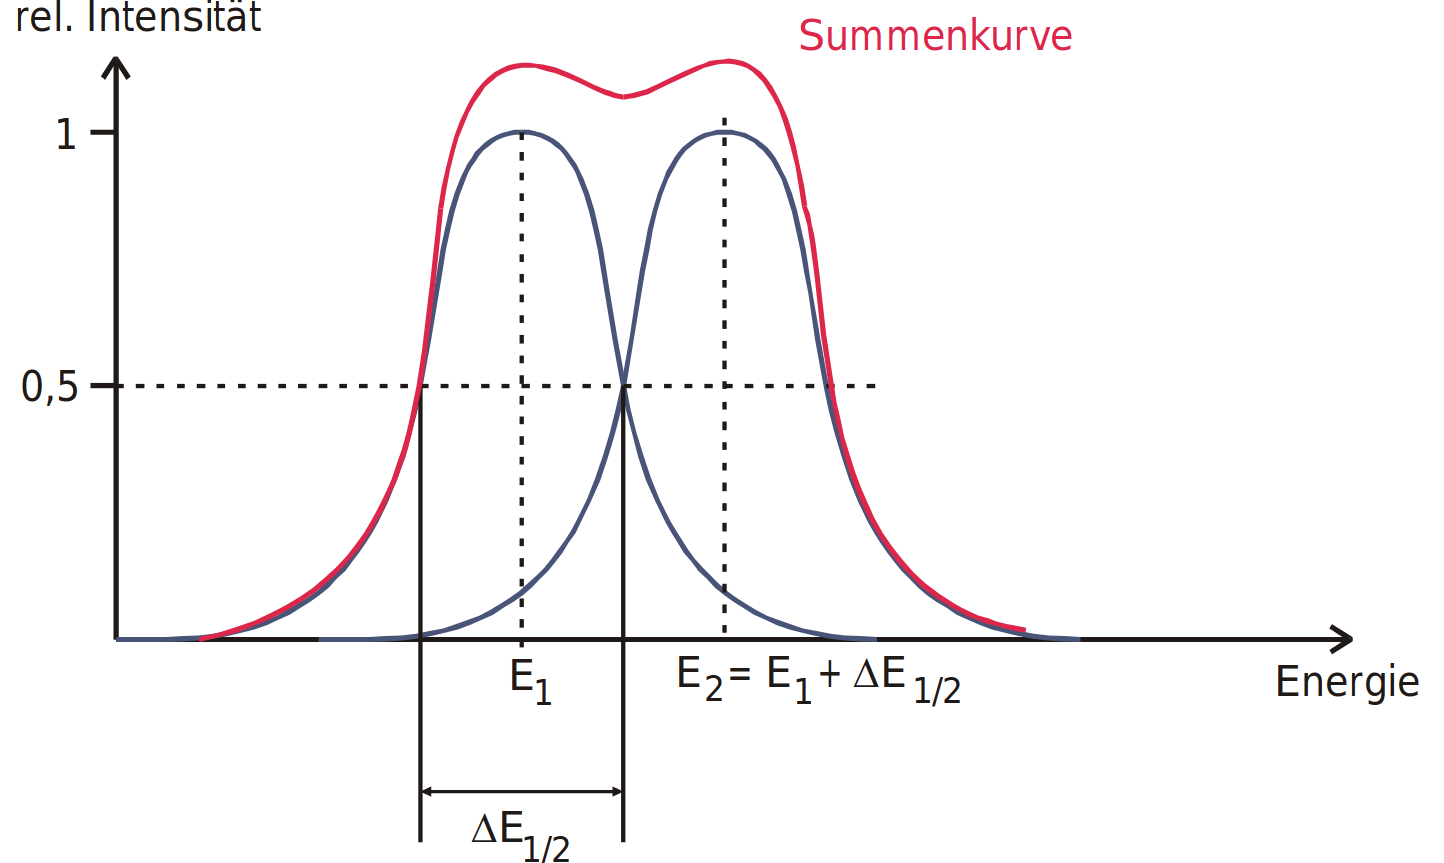
\includegraphics[width=0.8\textwidth]{Pics/energieaufloesung.png}
  \caption{Veranschaulichung der Halbwertsbreite als qualifizierendes Merkmal der Energieauflösung eine Detektors.
  Dargestellt sind zwei Peaks monochromatischer $\gamma$-Strahler im Energiespektrum mit den
  Mittelwerten $E_1$ und $E_2$\cite{anleitung}.}
  \label{fig:energieauflösung}
\end{figure}

Neben der Energieauflösung werden Detektoren bezüglich ihrer Vollenergienachweiswahscheinlichkeit
klassifiziert. Diese Vollenergienachweiswahscheinlichkeit $Q$
beschreibt wieviele eingefallene $\gamma$-Quanten von dem Detektor
registriert werden.
Die Vollenergienachweiswahscheinlichkeit wird mittels
\begin{equation}
  \label{eqn:effizienz}
  Q = \frac{4\pi}{\Omega}\frac{Z}{AW}
\end{equation}
berechnet. $\Omega$ ist der Raumwinkel, den der $\gamma$-Srahler vom Detektor abdeckt,
$A$ ist die Aktivität des Strahlers, $W$ die Emissionswahrschienlichkeit einer bestimmten
Energie eines Mehrlinienstrahlers und $Z$ die vom Detektor gezählten $\gamma$-Quanten
zu einer bestimmten Energie.
\FloatBarrier
\subsection{Energiespektren}
\label{subsec:energiespektrum}

Ein unendlich großer Detektor würde beim Ausmessen einer monochromatischen Probe mit~$E_\gamma$
lediglich im Energiespektrum einen scharfen Peak an der Stelle $E_\gamma$
ausgeben. Ein realer Detektor produziert hingegen ein Energiespektrum gemäß
Abbildung~\ref{fig:spektrum}. Dieses entsteht, da der Compton-Effekt
keine diskrete, sondern eine streuwinkelabhängige kontinuierliche Energieverteilung
erzeugt, die von der Nachweisgrenze bis zur Compton-Kante reicht.
Darüber hinaus entsteht ein Rückstreupeak aufgrund von größtenteils
außerhalb des Detektors rückgestreuten Photonen, welche mehrfach Compton-Streuung
machen.
Für die $\gamma$-Spektrometrie ist lediglich der Vollenergie-Peak
von Bedeutung, da in diesem die gesamte Energie des $\gamma$-Quants
in dem Detektor deponiert wird. Anhand der Vollenergiepeaks lässt
sich das ausgemessene Material eindeutig identifizieren.
Bei $\gamma$-Quantenergien kleiner als $\approx\SI{3}{\MeV}$ trägt lediglich der
Photoeffekt zu dem relevanten Vollenergie-Peak bei.

% Wird eine nicht-monochromatische Probe betrachtet kann der Compton-Effekt
% jedoch ebenfalls Beiträge zu einem Vollenergie-Peak leisten.
% Der Wirkungsquerschnitt des Compton-Effektes ist gemäß Abbildung~\ref{fig:crosssection}
% für Energien von $E_\gamma>\SI{0.15}{\MeV}$ größer als der Wirkungsquerschnitt
% der Photoeffektes, sodass es für diese Energien wahrscheinlicher ist, dass ein $\gamma$-Quant
% Energie über Compton-Streuung deponiert. Wenn dieses $\gamma$-Quant
% hinreichend viel Energie seiner anfänglichen Energie abgegeben hat,
% wird der Photoeffekt wahrscheinlicher, sodass es seine übrige Energie
% vollständig in dem Detektor deponieren kann.
% Aus diesem Grund wird der Peak nicht Photopeak, sondern Vollenergie-Peak genannt.

\begin{figure}
  \centering
  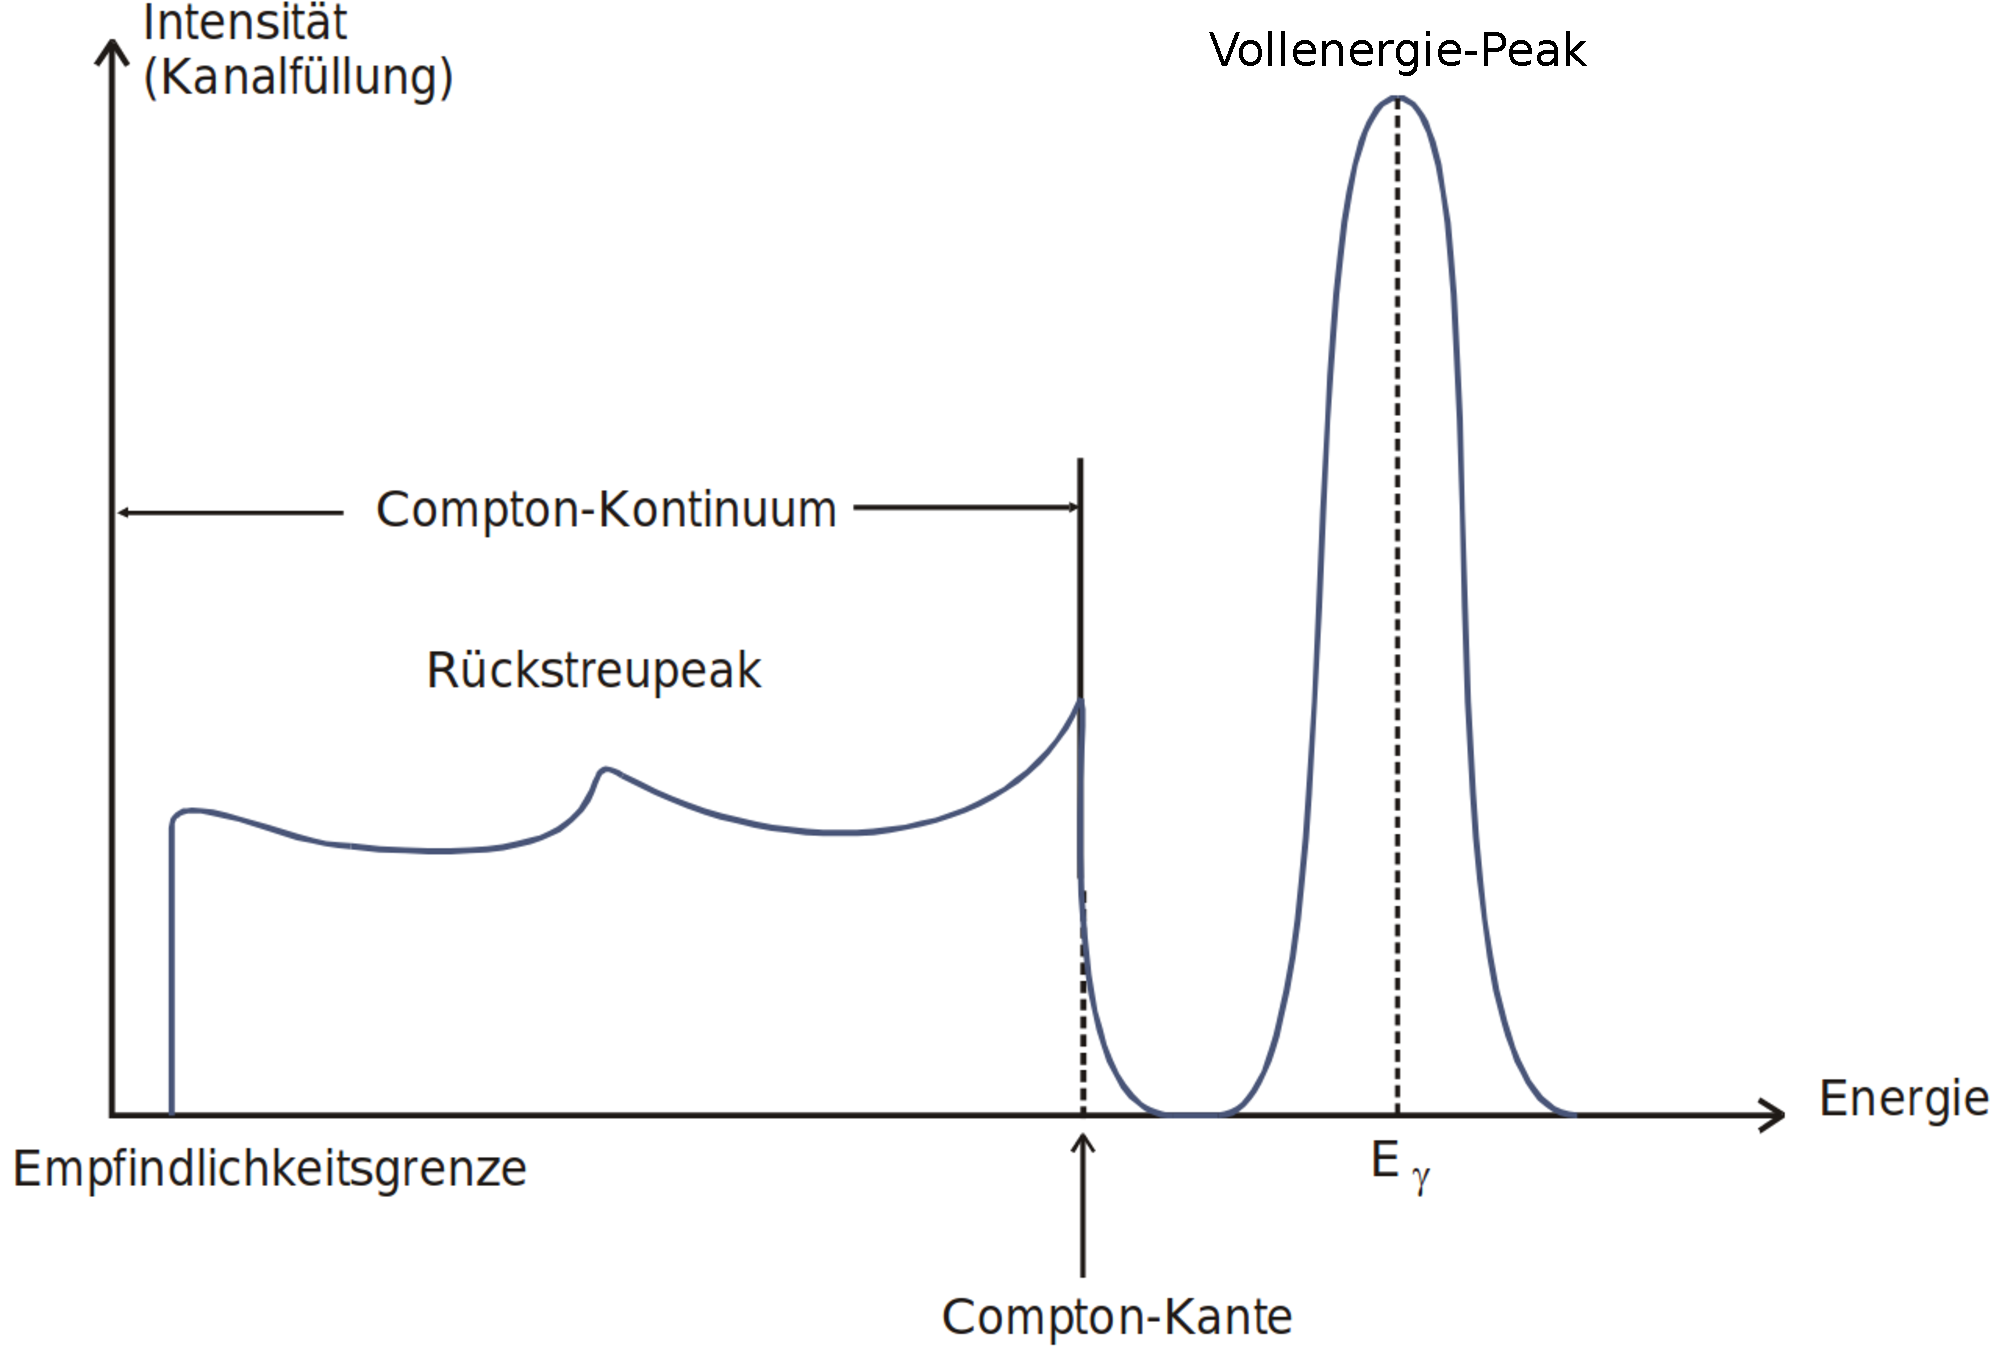
\includegraphics[width=0.8\textwidth]{Pics/spektrum.pdf}
  \caption{Gemessenens Energiespektrum einer monochromatischen Quelle (nach Quelle~\cite{anleitung}).}
  \label{fig:spektrum}
\end{figure}
\FloatBarrier
\section{Aufbau}
\label{sec:Aufbau}

Der grundlegende Aufbau ist in Abbildung~\ref{fig:aufbau} gezeigt. Der Detektor
besteht aus einem hochreinen Germanium-Kristall, welcher im Inneren eine
koaxiale Bohrung hat, die mit Gold bedampft ist.
Die Außenseite des Germanium-Kristalls ist mit Lithium dotiert,
sodass diese gut leitend ist. Die Li-Schicht dient als Pluspol der Sperrspannung $U$.\\
Der Detektor ist mit einer Aluminiumschicht ummantelt, welche als mechanischer
Schutz und zur thermischen Entkopplung von der Umgebung fungiert. Als Abschirmung
vor natürlicher Strahlung um die Aluminiumschicht eine Kupferschicht und eine Bleischicht angebracht.
Die Bleischicht eignet sich aufgrund ihrer hohen Dichte besonders gut als Abschirmungsmaterial
für jegliche Strahlung.
Die $\ce{Cu}$-Schicht schirmt Strahlung von $\ce{Pb}$-Isotopen aus dem Blei ab.

\begin{figure}
  \centering
  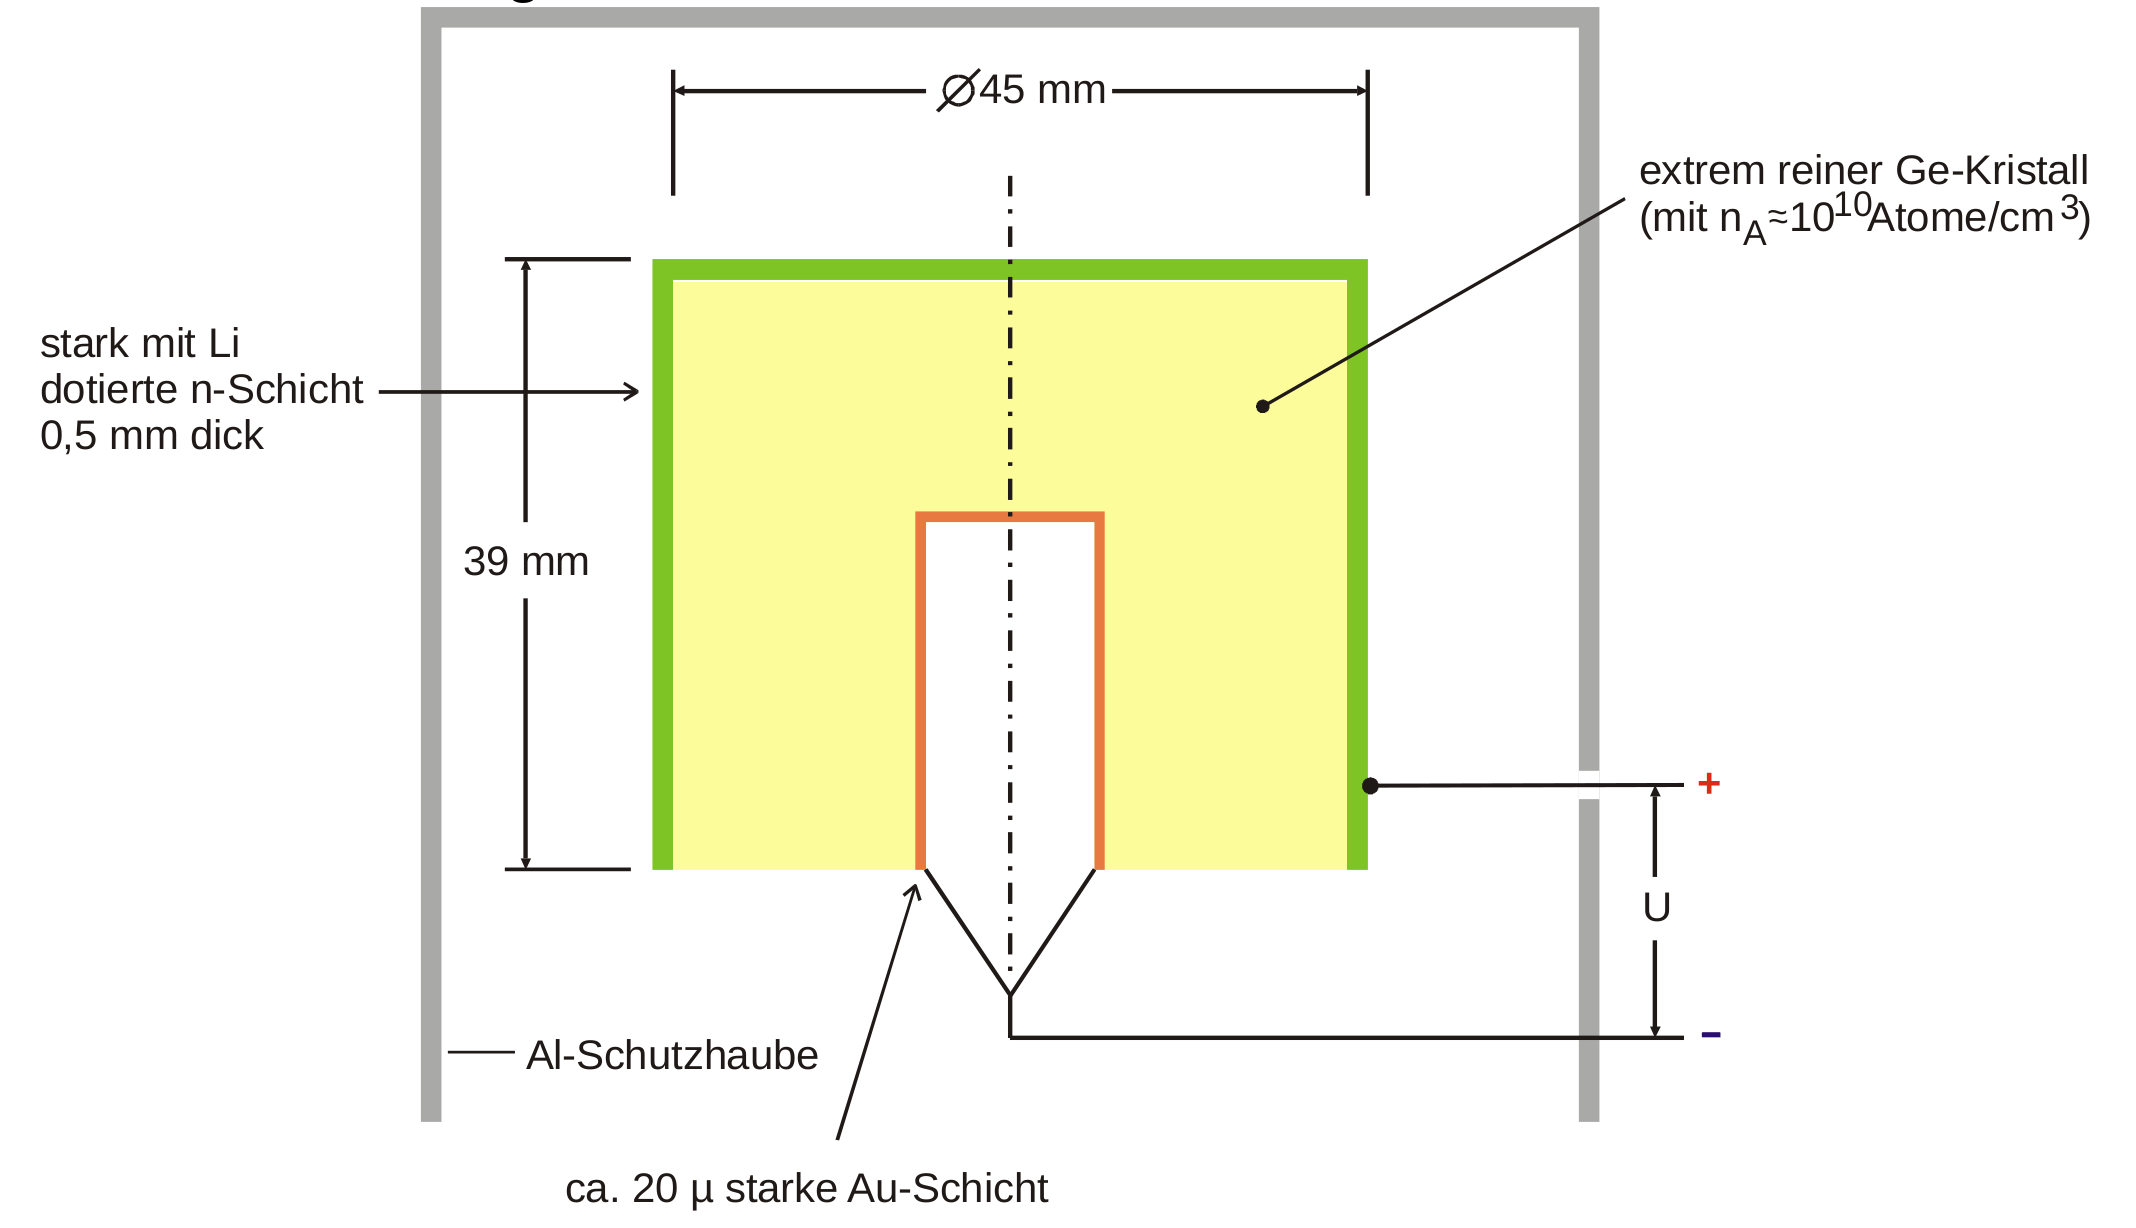
\includegraphics[width=0.85\textwidth]{Pics/aufbau.png}
  \caption{Schematischer Aufbau eines $\ce{Ge}$-Detektors. Nicht eingezeichnet sind
  die den gesamten Detektor umschließenden Abschirmungsschichten aus Kupfer und Blei\cite{anleitung}.}
  \label{fig:aufbau}
\end{figure}
\FloatBarrier
\subsection{Elektronische Beschaltung eines $\ce{Ge}$-Detektors}
\label{subsec:elektronische}

Das Ziel der elektronischen Beschaltung ist es die im Detektor deponierte
Energie der gemessenen $\gamma$-Quanten in ein elektronisch auswertbares
Signal um zu wandeln.
Damit ein Energiespektrum erstellt werden kann, müssen die vom Detektor gemessenen
$\gamma$-Quanten ihrer Energie entsprechend in die Höhe von Spannungsimpulse übersetzt werden.
Dafür wird der in Abbildung~\ref{fig:vorverstärker} gezeigte Vorverstärker verwendet.
Dieser wandelt die Ladungsmenge, die das $\gamma$-Quant in dem Detektor freisetzt
über eine Integrationsschaltung in einen Spannungsimpuls um.

\begin{figure}
  \centering
  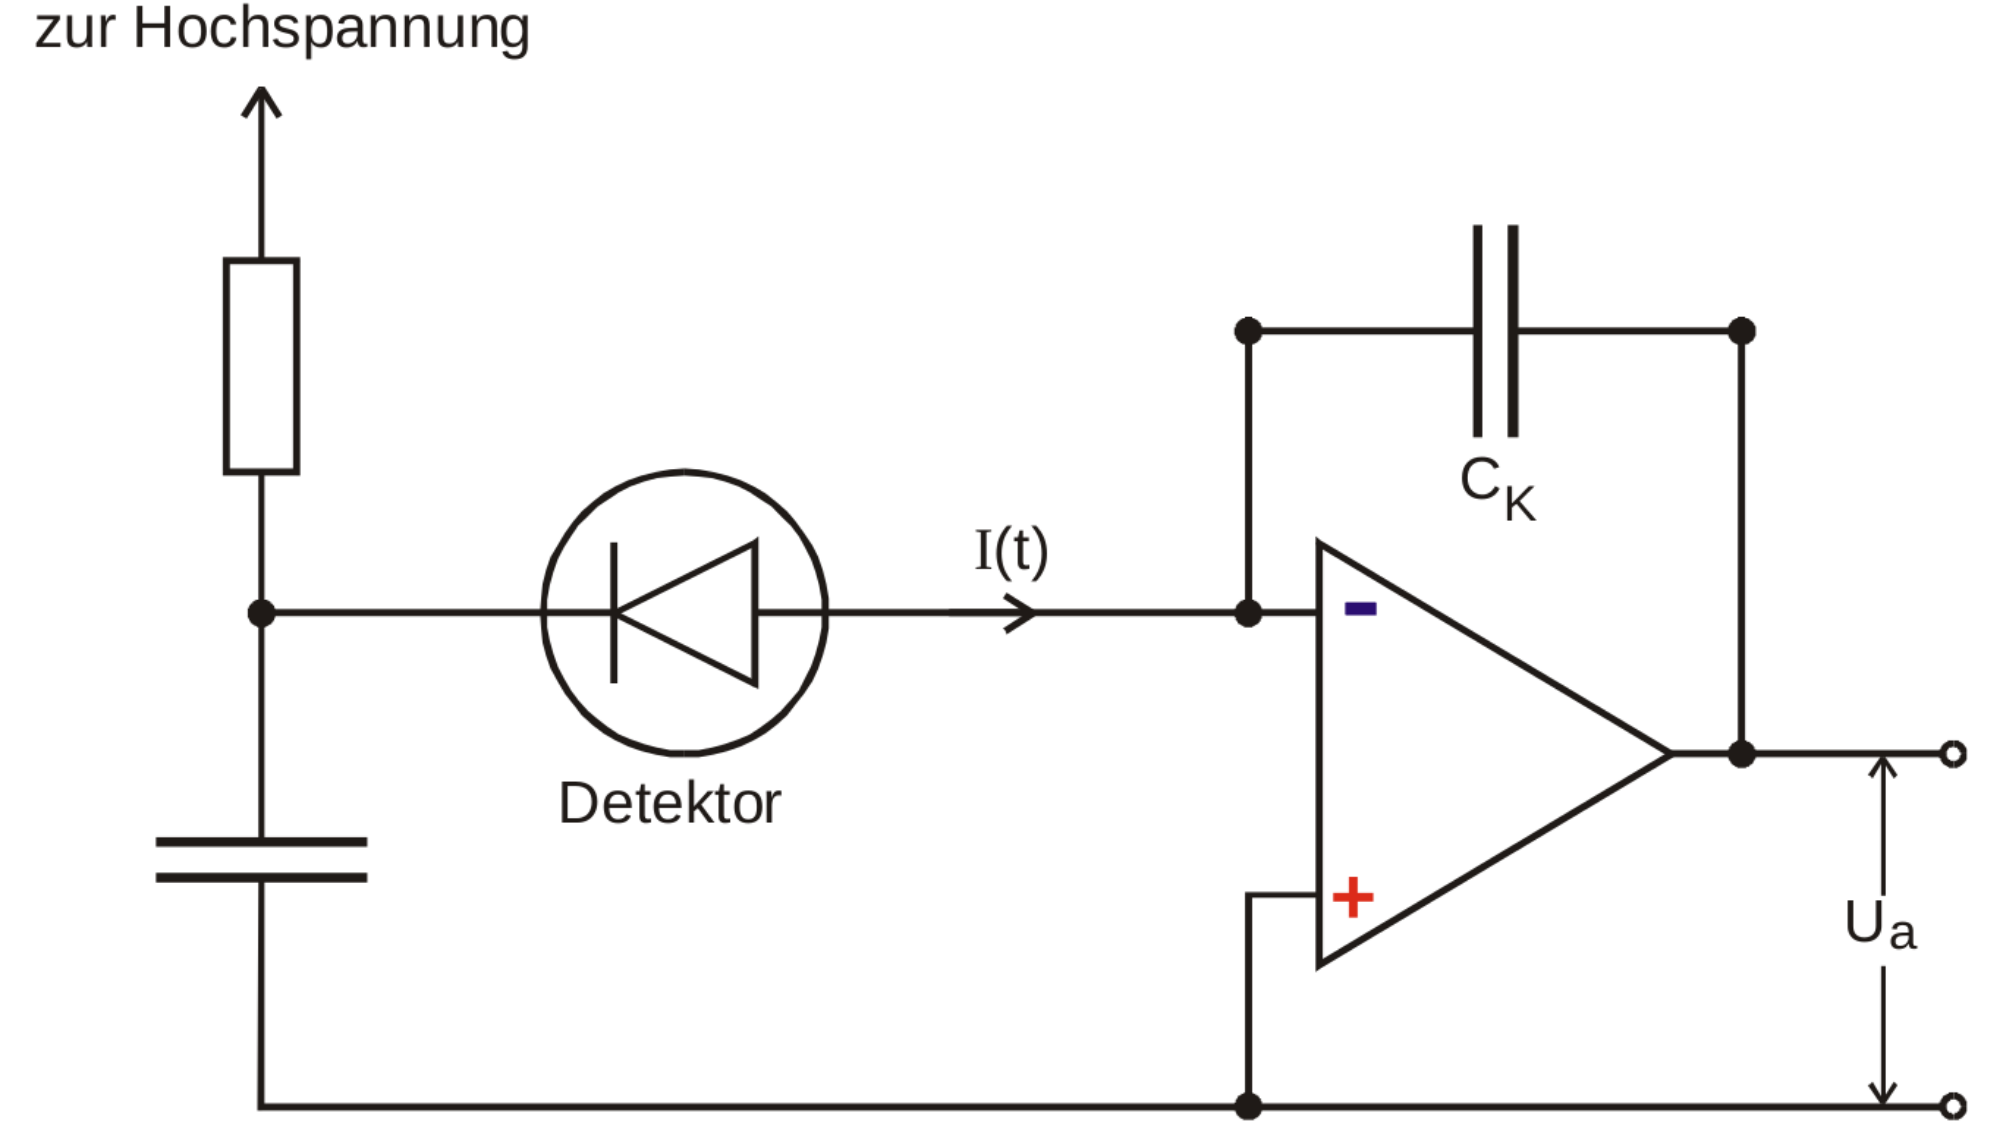
\includegraphics[width=0.6\textwidth]{Pics/vorverstaerker.png}
  \caption{Schaltungsskizze eines Vorverstärkers für den $\ce{Ge}$-Detektor\cite{anleitung}.}
  \label{fig:vorverstärker}
\end{figure}

Nach jedem Quantennachweis muss der Integrationskondensator $C\ua{K}$ aus Abb.~\ref{fig:vorverstärker}
entladen werden, damit der korrekte Zusammenhang zwischen $E_\gamma$ und
der Entladungszeit $t_s$ des Kondensators für jeden Nachweis sichergestellt ist.
Das Entladen kann über den in Abb.~\ref{fig:vorverstärker} gestrichelt eingezeichneten
Widerstand $R\ua{K}$ gelöst werden. Problematisch ist jedoch das Eigenrauschen des
Widerstands, welches das Rauschen des Vorverstärkers signifikant beeinträchtigt.
Zur Entladung des Kondensator wird aus diesem Grund eine optoelektronische
Rückkoplung verwendet. Eine solche Schaltung ist schematisch in Abb.~\ref{fig:optoelektronik}
gezeigt. Nach jedem Nachweis wird ein Eingangs-Feldeffekttransistor (FET)
mittels einer LED beleuchtet, sodass die Sperrschicht für eine kurze Zeit leitend wird.
Die Ladung kann dann über den Integrationskondensator abfließen.

\begin{figure}
  \centering
  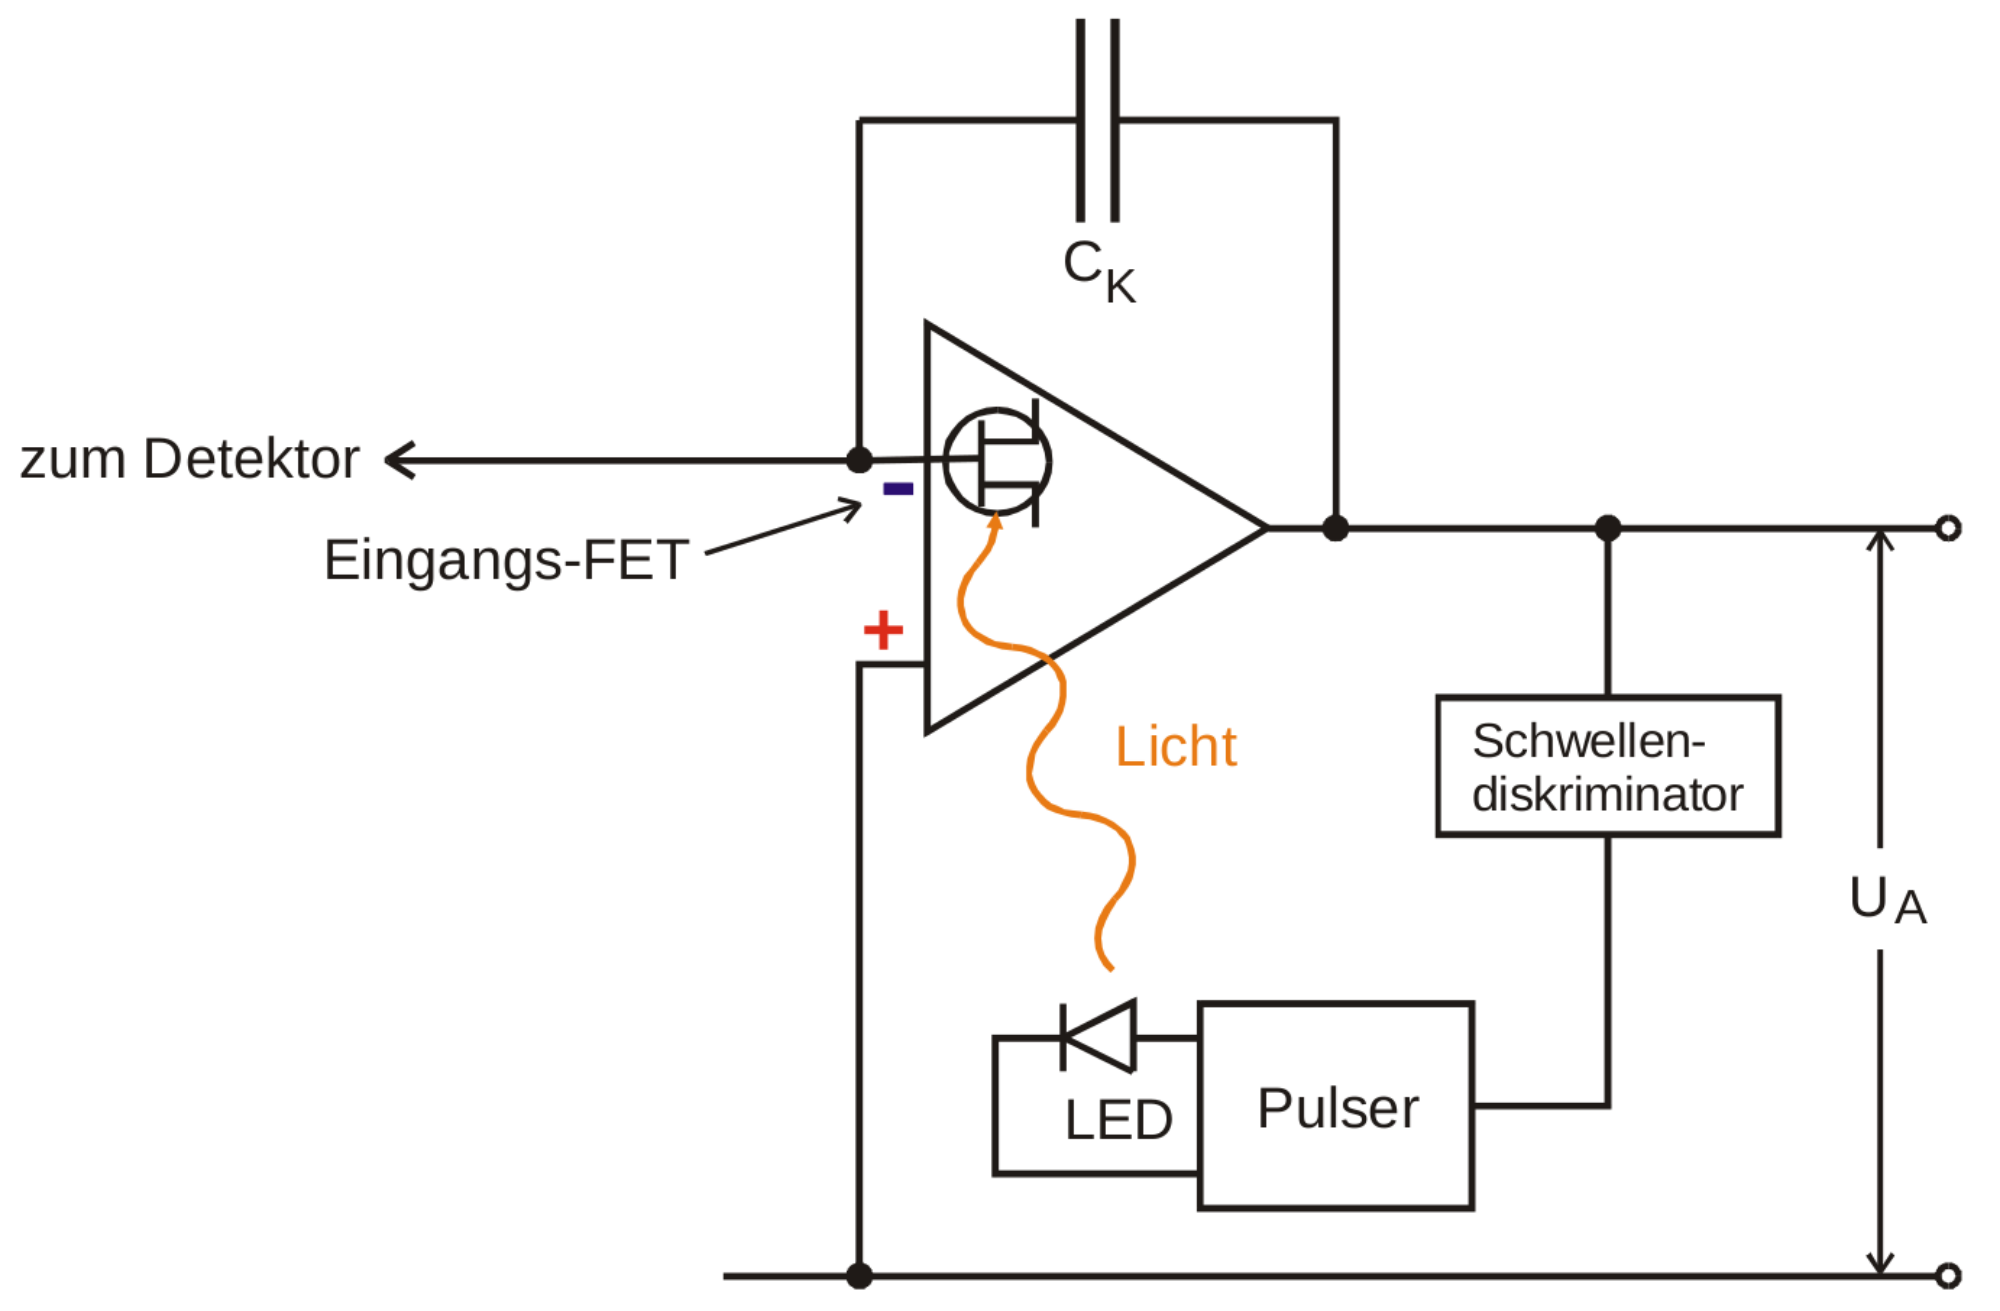
\includegraphics[width=0.6\textwidth]{Pics/optoelektronik.png}
  \caption{Schaltungsskizze zur Entladung des Integrationskondensators $C\ua{K}$ durch optoelektronische Rückkoplung\cite{anleitung}.}
  \label{fig:optoelektronik}
\end{figure}

Die aus dem Vorverstärker kommenden Spannungsimpulse werden meinst
über ein $RC$-Glied ($R\ua{Verbindung}$ und $C\ua{Verbindung}$)
mit dem Hauptverstärker verbunden.
Der Hauptverstärker wandelt das Signal des Vorverstärkers in einen
Gaußpuls um. Dieser Gaußpuls besitzt dieselbe Fläche wie die
Entladungskurve des Vorverstärkers.
Die Verbindung des Vor- und des Hauptverstärkers kann aufgrund
der verschiedenen Abklingkonstanten der $RC$-Glieder $R\ua{K}C\ua{K}$
und $R\ua{Verbindung}C\ua{Verbindung}$ Unterschwinger hervorrufen.
Diese Unterschwinger verschlechtern die Energieauflösung,
da einem während eines Unterschwinger eintreffenden Impulses
eine zu kleine Spannungsamplitude im Hauptverstärker zugeordnet werden
würde. Mit Hilfe einer \emph{Pole-Zero}-Kompensation lassen sich
die unerwünschten Unterschwinger unterdrücken.
Die \emph{Pole-Zero}-Kompensation wird erreicht, wenn ein geeigneter
Anteil der Gleichspannung aus dem Vorverstärker das $RC$-Glied
umgeht.
Darüber hinaus beinhaltet der Hauptverstärker eine \emph{Base-Line-Restorer}-Schaltung,
welche das Absinken der Nullinie am Ausgang des Hauptverstärkers verhindert.
Ein sogenannter Viel-Kanal-Analysator (VKA)
nimmt die Gaußspulse entgegen, und ordned deren Höhe, welche stellvertretend für die
Energie des $\gamma$-Quantes steht, entsprechend in die vorhandenen Kanäle ein.
Diese Einordnung geschieht über ein Adressregister, das
digitale Signale von dem Analog-Digital-Konverter (ADC) erhält.
Der ADC sorgt dafür, dass die Spannungsimpulshöhe des Gaußpeaks
in eine dazu proportionales Digitalsignal übersetzt wird.
Der Viel-Kanal-Analysator wird durch einen Computer mit geeigneter Software
ausgelesen. Die Kanäle des VKAs sind nicht kalibriert.

Treffen mehrere $\gamma$-Quanten innerhalb kurzer Zeit in den Detektor,
kann es zur fälschlichen Erhöhung des Signale kommen,
wodurch eine zu hohe $\gamma$-Quantenenergie gemessen wird.
Diese Erhöhung wird in der Literatur als \emph{pile-up} bezeichnet und
wird durch sogenannte Pile-up-Rejection-Schaltungen (PUR) unterdrückt.
Die PUR sperrt den Eingang des Analog-Digial-Konverters, sodass
diese \emph{pile-up}-Signale nicht im Spektrum auftauchen.


% \begin{figure}
%   \centering
%   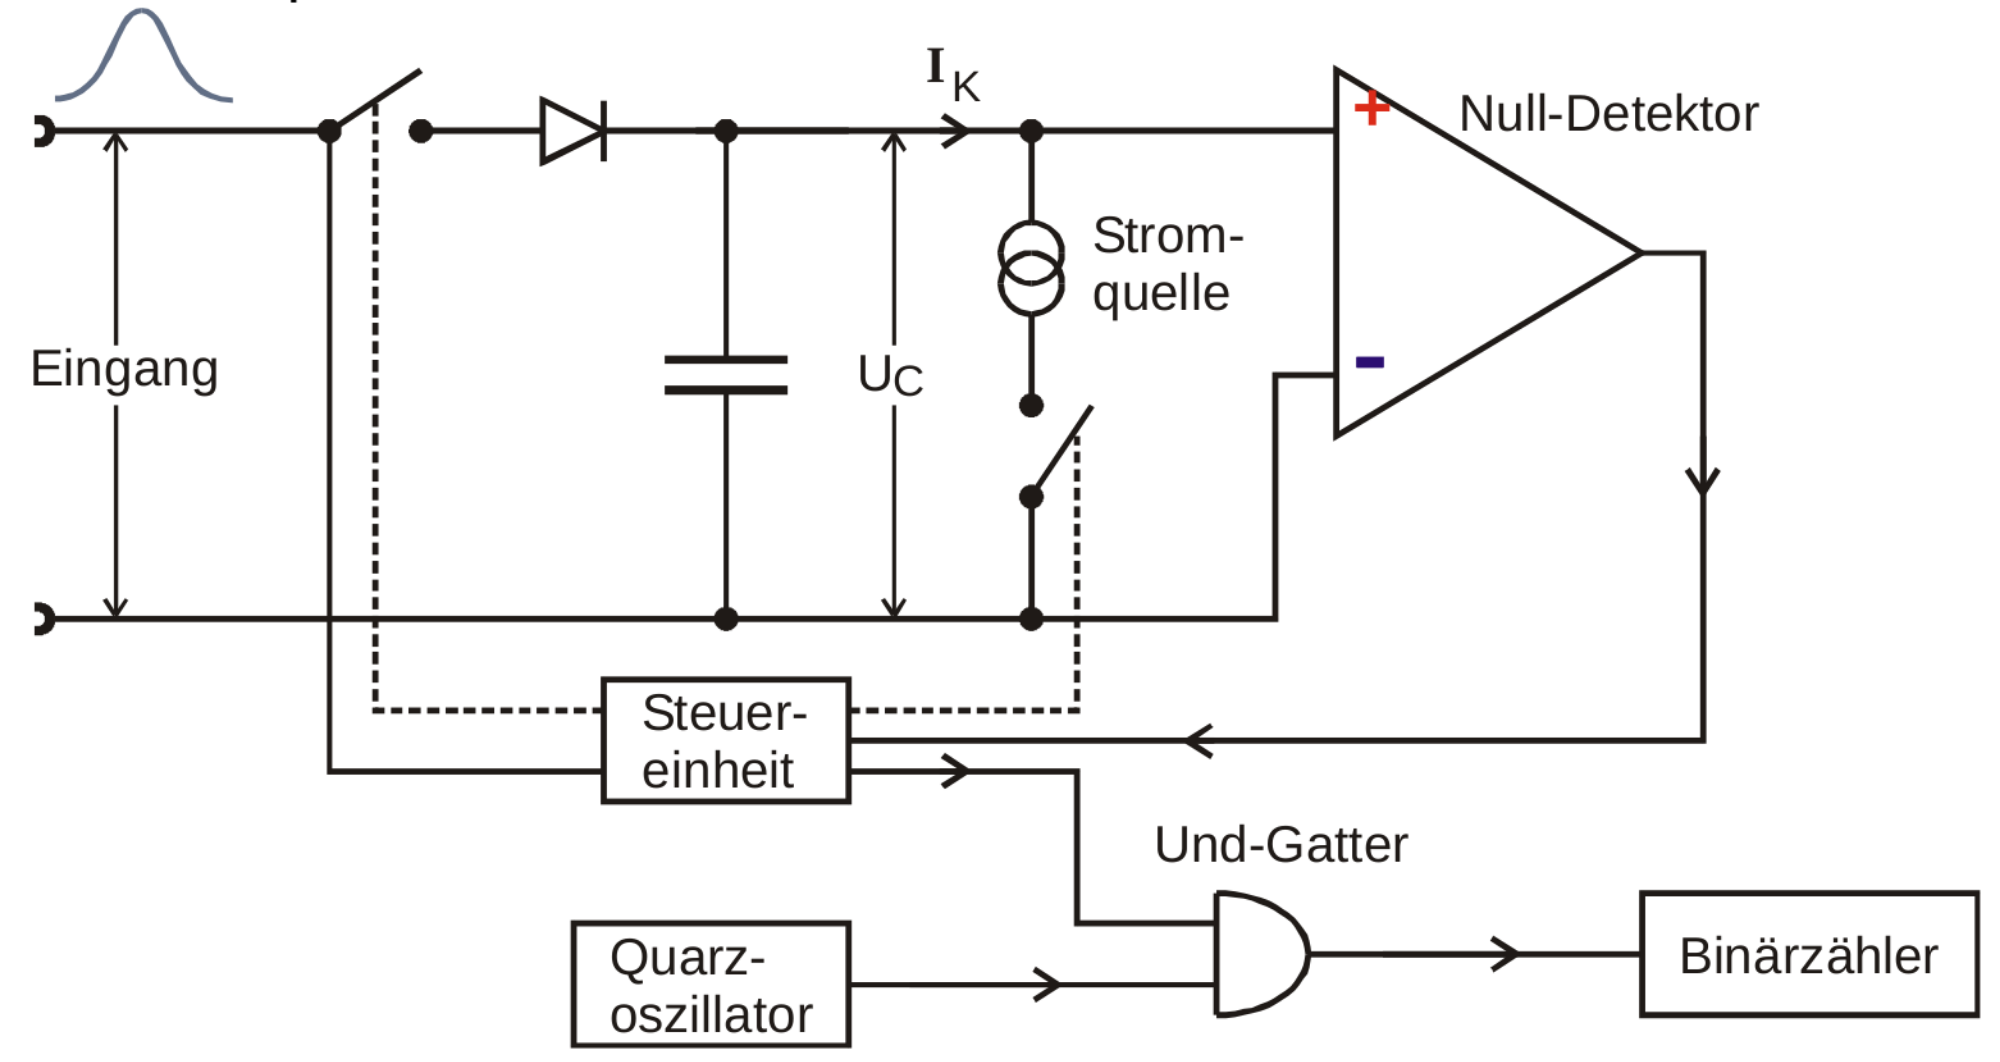
\includegraphics[width=0.8\textwidth]{Pics/WAD_konverter.png}
%   \caption{Prinzipschaltbild eines Wilkinson-Analog-Konverters\cite{anleitung}.}
%   \label{fig:konverter}
% \end{figure}
\FloatBarrier
\section{Durchführung}
\label{sec:durchführung}

Zu Beginn des Versuches wird eine bekannte Probe zum Kalibieren der Eingänge des
Viel-Kanal-Analysators und der Vollenergienachweiswahscheinlichkeitsmessung
vewendet. Dafür wird ein $\ce{^152Eu}$-Strahler verwendet.
Weiterhin wird ein $\ce{^137Cs}$-Strahler zur Bestimmung weiterer Detektoreigenschaften
ausgemessen.\\
Abschließend werden zwei unbekannte Strahler vermessen, die anhand ihrers
Energiespektrums identifiziert werden.
